\section{Theoretical Analysis}
\label{sec:analysis}

In this section, the circuit shown in Figure~\ref{fig:T2Circuit} is analysed theoretically in six steps.

In step (1), first of all, we used the nodal method to determine the voltages in all nodes and currents in all branches for t<0. The results are shown in Table~\ref{tab:TA1}.

\begin{table}[h]
  \centering
  \begin{tabular}{|l|r|}
    \hline    
    {\bf Nodes and branches} & {\bf Value [V]/[A]} \\ \hline
    v1 & 5.134164 \\ \hline
v2 & 4.929601 \\ \hline
v3 & 4.510168 \\ \hline
v4 & 0.000000 \\ \hline
v5 & 4.957651 \\ \hline
v6 & 5.588276 \\ \hline
v7 & -2.095712 \\ \hline
v8 & -3.151534 \\ \hline
  \end{tabular}
  \caption{Theoretical voltage values for each node, expressed in Volt, and current values for each branch, expressed in Ampere.}
  \label{tab:TA1}
\end{table}

After this, in step (2), we determined the equivalent resistance as seen from the capacitor terminals. In order to do so, we followed the professor's sugestion: ... The computed results can be found in Table~\ref{tab:TA2}.

\begin{table}[h]
  \centering
  \begin{tabular}{|l|r|}
    \hline    
    {\bf Computed Results} & {\bf Values} \\ \hline
    v1 & 0.000000 \\ \hline
v2 & 0.000000 \\ \hline
v3 & 0.000000 \\ \hline
v4 & 0.000000 \\ \hline
v5 & 0.000000 \\ \hline
v6 & 8.739810 \\ \hline
v7 & 0.000000 \\ \hline
v8 & 0.000000 \\ \hline
Ix & -0.002826 \\ \hline
Vx & 8.739810 \\ \hline
Req & -3092.796241 \\ \hline
  \end{tabular}
  \caption{Computed results: voltage expressed in Volt, current in Ampere and resistence in Ohm.}
  \label{tab:TA2}
\end{table}

Later, in step (3), we used the value of the equivalent resistant calculated in point (2) to find the natural solution of v6. Knowing that "\tau" is calculated multiplying Req with C(capacitance of the capacitor), in Equation~\ref{eq:natsol} we find the formula required to calculate the natural solution we wanted. 

\begin{equation}
  V_{6n}(t) = V_{x}e^{-\frac{t}{\tau}},
  \label{eq:natsol}
\end{equation}

Also the solution is ploted in Figure~\ref{figure:plotA(4)} where the x-axis corresponds to time, 't', expressed in [ms] and the y-axis corresponds to the natural solution of v6, 'v6n', expressed in [V].

\begin{figure}[h] \centering
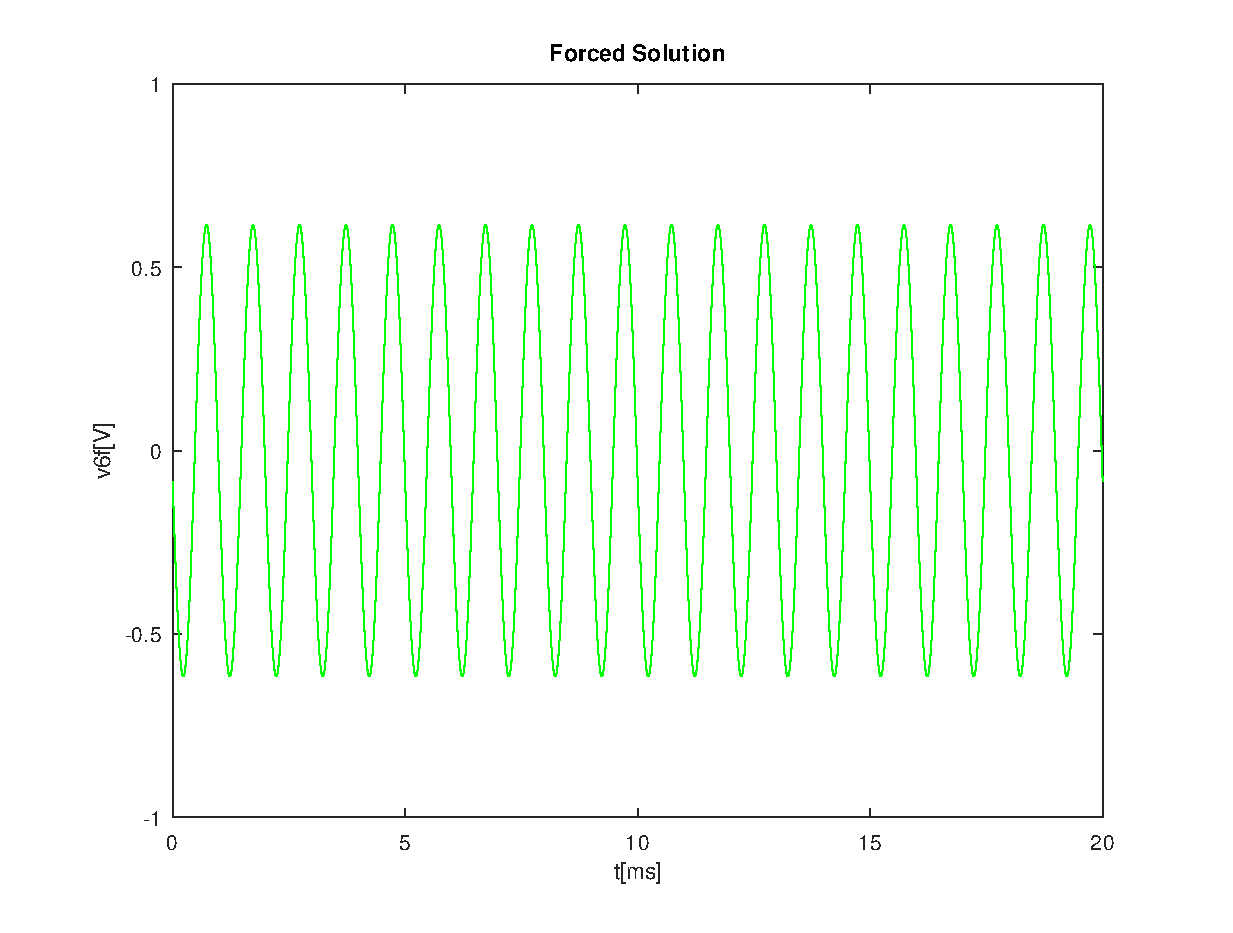
\includegraphics[width=0.8\linewidth]{forced_solution.eps}
\caption{Plot of v6n(t) in the interval [0, 20]ms.}
\label{fig:plotA(4)}
\end{figure}

In step (4), the forced solution v6f(t) was determined for f=1KHz and for 't' in the interval [0,20]ms. Moreover, the capacitance was replaced by the impedance, 'Z', and Vs was considered equal to one. The complex amplitudes in the nodes are shown in Table~\ref{tab:TA4}.

\begin{table}[h]
  \centering
  \begin{tabular}{|l|r|}
    \hline    
    {\bf Nodes} & {\bf Complex Amplitudes} \\ \hline
    |v1| & 1.000000 \\ \hline
|v2| & 0.960156 \\ \hline
|v3| & 0.878462 \\ \hline
|v4| & 0.000000 \\ \hline
|v5| & 0.965620 \\ \hline
|v6| & -0.609606 \\ \hline
|v7| & -0.408190 \\ \hline
|v8| & -0.613836 \\ \hline
  \end{tabular}
  \caption{Complex amplitudes in the nodes, expressed in Volt.}
  \label{tab:TA4}
\end{table}






